\documentclass[12pt, letterpaper, twoside]{article}
\usepackage{nopageno,epsfig, amsmath, amssymb}
\usepackage{physics}
\usepackage{mathtools}
\usepackage{hyperref}
\usepackage{xcolor}
\hypersetup{
    colorlinks,
    linkcolor={blue},
    citecolor={blue},
    urlcolor={blue}
}
\usepackage{empheq}
\usepackage{wrapfig}

\usepackage[letterpaper,
            margin=0.8in]{geometry}

\newcommand{\psetnum}{1}
\newcommand{\class}{ASTR 581 - Observing}

\newcommand{\tomtitle}{
    \noindent {\LARGE \fontfamily{cmr}\selectfont \textbf{\class}} \hfill \\[1\baselineskip]
    \noindent {\large \fontfamily{cmr}\selectfont Observing Planning \hfill \textsc{Tom Wagg}}\\[0.5\baselineskip]
    {\fontfamily{cmr}\selectfont \textit{\today}}\\[2\baselineskip]
}

\title{\class : Observing Planning}
\author{\textbf{Tom Wagg}}

\newcommand{\question}[1]{{\noindent \it #1}}
\newcommand{\answer}[1]{
    \par\noindent\rule{\textwidth}{0.4pt}#1\vspace{0.5cm}
}
\newcommand{\todo}[1]{{\color{red}\begin{center}TODO: #1\end{center}}}

% custom function for adding units
\makeatletter
\newcommand{\unit}[1]{%
    \,\mathrm{#1}\checknextarg}
\newcommand{\checknextarg}{\@ifnextchar\bgroup{\gobblenextarg}{}}
\newcommand{\gobblenextarg}[1]{\,\mathrm{#1}\@ifnextchar\bgroup{\gobblenextarg}{}}
\makeatother

\newcommand{\avg}[1]{\left\langle #1 \right\rangle}
\newcommand{\angstrom}{\mbox{\normalfont\AA}}
\allowdisplaybreaks

\begin{document}

\tomtitle

\noindent I use astroplan/astropy throughout. You can see my code here: \url{https://github.com/TomWagg/uw-grad-classes/tree/main/581_observing/observing_planning/code.ipynb}\\

\question{1. APO Location}
\answer{
    Latitude: 32.7803 degrees North\\
    Longitude: 105.8203 degrees West
}

\question{2. APO Sunset}
\answer{
    Sunset is at 01:01 UTC and 19:01 MST.
}

\question{3. Sidereal Time}
\answer{
    Honestly a little confused on this because astropy gave me an hour angle but I \textit{think} the time is 23:23:16.
}

\question{4. Moon Phase}
\answer{
    Waning Crescent
}

\question{5. Moon time}
\answer{
    06:49 UTC
}

\question{6. Moon inteference}
\answer{
    I think it depends. The moon is waning crescent so it's not too bright, and it doesn't rise until the B half so A half observations won't be affected. For the B half it will depend on the separation of the target from the moon and how bright it is.
}

\clearpage

\question{7. RA/Dec of objects}
\answer{
    M91: (88.859260, +14.4958754)\\
    NGC 5866: (26.6231708, +55.7633927)
}

\question{8. Observable from MRO}
\answer{
    Only NGC 5866 is observable at this time of year
}

\question{9. Airmass conditions}
\answer{
    NGC 5866 will only have an airmass less than 1.5 for about 30 minutes after sunset (before twilight) so it may be difficult to see.
}

\begin{figure}[htb]
    \centering
    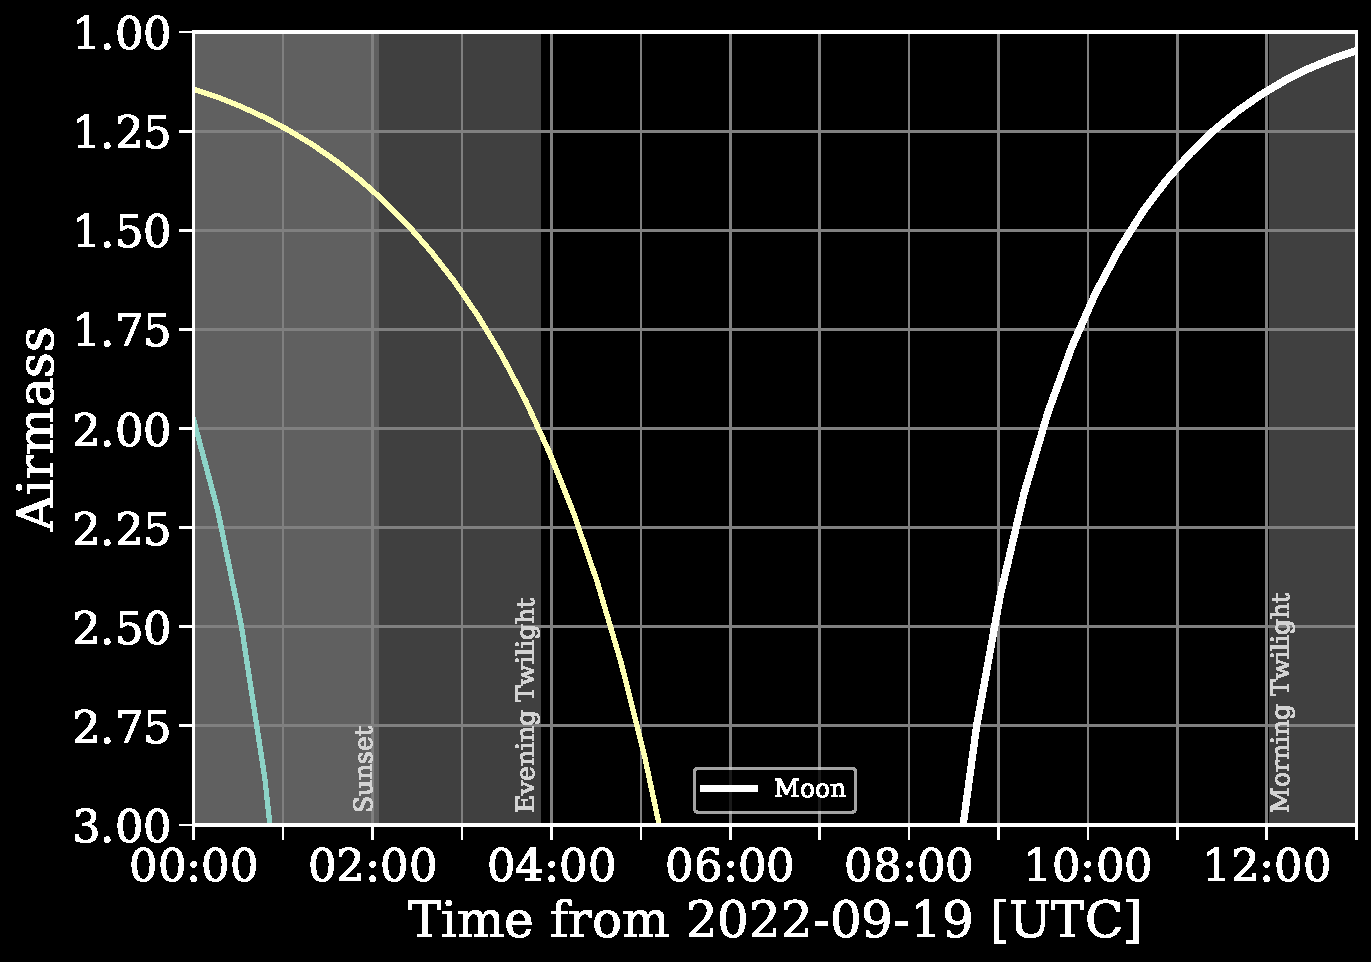
\includegraphics[width=0.7\textwidth]{mro_galaxies.pdf}
\end{figure}

\question{10. Morning twilight}
\answer{
    Astronomial morning twilight occurs at 12:02:20 UTC so any time after that you'll start struggling to see fainter sources.
}

\question{11. Best seasons to observe}
\answer{
    March is best for M91, and May is best for NGC 5866. These months maximise the time this object spends with airmass $< 1.5$ at MRO.
}

\question{12. Dust?}
\answer{
    No need to worry. These objects have galactic latitudes of 76.82963912 and 52.5908177 degrees so they are far from the galactic plane.
}

\end{document}
